\documentclass[12pt]{article}

\usepackage[a4paper,top=1in,bottom=1in,left=1in,right=1in]{geometry}

\usepackage[utf8]{inputenc}
\usepackage{float}
\usepackage{amsmath}
\usepackage{graphicx}
\usepackage{titlesec}
\usepackage{tcolorbox}
\usepackage{enumitem}
\usepackage{tikz}
\usepackage{tikz-timing}
\usetikzlibrary{patterns}
\usetikzlibrary{graphs}
\usetikzlibrary{graphdrawing}
\usegdlibrary{force}
\usepackage{amssymb}
\usepackage{hyperref}

\title{\bfseries Laborator Proiectare Logică 10}
\author{Sîrghe Matei}
\date{January 9, 2025}

\titleformat{\section}
  {\normalfont\Large\bfseries}{\thesection}{1em}{}
\begin{document}
\maketitle

\renewcommand{\arraystretch}{1}

Avem un numărător:

\begin{figure}[h!]
    \begin{minipage}{0.45\textwidth}
        \begin{tikzpicture}
            \node[circle, draw] (A) at (0,0) {000};
            \node[circle, draw] (B) at (-2,-1) {111};
            \node[circle, draw] (C) at (0,-2) {010};
            \node[circle, draw] (D) at (2,-1) {100};
            \node[circle, draw] (E) at (0,-3.5) {110};
            \node[circle, draw] (F) at (0,-5) {101};
            \node[circle, draw] (G) at (-2,-6.5) {001};
            \node[circle, draw] (H) at (2,-6.5) {011};
            
            \draw[->] (A) -- (C);
            \draw[->] (B) -- (C);
            \draw[->] (D) -- (C);
            \draw[->] (C) -- (E);
            \draw[->] (E) -- (F);
            \draw[->] (F) -- (H);
            \draw[->] (H) -- (G);
            \draw[->] (G) -- (F);
        \end{tikzpicture}  
    \end{minipage}
    \hfill
    \begin{minipage}{0.45\textwidth}
        \begin{tabular}{|c|c|c|c|c|c|}
            \hline
            $Q_2$ & $Q_1$ & $Q_0$ & $Q_{2}^{'}$ & $Q_{1}^{'}$ & $Q_{0}^{'}$ \\ \hline
            0 & 0 & 0 & 0 & 1 & 0 \\ \hline
            0 & 0 & 1 & 1 & 0 & 1 \\ \hline
            0 & 1 & 0 & 1 & 1 & 0 \\ \hline
            0 & 1 & 1 & 0 & 0 & 1 \\ \hline
            1 & 0 & 0 & 0 & 1 & 0 \\ \hline
            1 & 0 & 1 & 0 & 1 & 1 \\ \hline
            1 & 1 & 0 & 1 & 0 & 1 \\ \hline
            1 & 1 & 1 & 0 & 1 & 0 \\ \hline
        \end{tabular}
    \end{minipage}
\end{figure}  

\begin{figure}[h!]
    \begin{minipage}{0.32\textwidth}
        \begin{tikzpicture}
            \draw (0,0) grid (4,-2);
            \draw[-] (0,0) -- (-1,1);
            \node at (-0.75, 1.25) {$Q_2$};
            \node at (-0.75, 0.25) {$Q_1$};
            \node at (-0.25, 0.75) {$Q_0$};

            \draw (0,0) grid (4,-2);
        
            \draw[thick] (2, -0.5) ellipse (1cm and 0.5cm);
            \draw[thick] (0.5, -1.5) ellipse (0.5cm and 0.5cm);
        
            %\draw[thick] (4,-3) arc[start angle=90, end angle=180, x radius=1cm, y radius=1cm];

            \node at (0.5, -0.5) {0};
            \node at (1.5, -0.5) {1};
            \node at (2.5, -0.5) {1};
            \node at (3.5, -0.5) {0};
            %
            \node at (0.5, -1.5) {1};
            \node at (1.5, -1.5) {0};
            \node at (2.5, -1.5) {0};
            \node at (3.5, -1.5) {0};
            
            \node at (0.5, 0.5) {00};
            \node at (1.5, 0.5) {01};
            \node at (2.5, 0.5) {11};
            \node at (3.5, 0.5) {10};
        
            \node at (-0.5, -0.5) {00};
            \node at (-0.5, -1.5) {01};
        \end{tikzpicture}
    \end{minipage}
    \hfill
    \begin{minipage}{0.65\textwidth}
        \[
        \begin{cases}
        D_2=Q_2^{'} \\
        D_1=Q_1^{'} \\
        D_0=Q_0^{'} \\ 
        D_2=Q_1\bar{Q_0}+\bar{Q_2}\bar{Q_1}Q_0
        \end{cases}
        \]
    \end{minipage}
\end{figure}  

\begin{figure}[h!]
    \begin{minipage}{0.32\textwidth}
        \begin{tikzpicture}
            \draw (0,0) grid (4,-2);
            \draw[-] (0,0) -- (-1,1);
            \node at (-0.75, 1.25) {$Q_2$};
            \node at (-0.75, 0.25) {$Q_1$};
            \node at (-0.25, 0.75) {$Q_0$};

            \draw (0,0) grid (4,-2);
        
            \draw[thick] (1, -0.5) ellipse (1cm and 0.5cm);
            \draw[thick] (3, -1.5) ellipse (1cm and 0.5cm);
            \draw[thick] (3.5, -1) ellipse (0.5cm and 1cm);
        
            %\draw[thick] (4,-3) arc[start angle=90, end angle=180, x radius=1cm, y radius=1cm];

            \node at (0.5, -0.5) {1};
            \node at (1.5, -0.5) {1};
            \node at (2.5, -0.5) {0};
            \node at (3.5, -0.5) {1};
            %
            \node at (0.5, -1.5) {0};
            \node at (1.5, -1.5) {0};
            \node at (2.5, -1.5) {1};
            \node at (3.5, -1.5) {1};
            
            \node at (0.5, 0.5) {00};
            \node at (1.5, 0.5) {01};
            \node at (2.5, 0.5) {11};
            \node at (3.5, 0.5) {10};
        
            \node at (-0.5, -0.5) {00};
            \node at (-0.5, -1.5) {01};
        \end{tikzpicture}
    \end{minipage}
    \hfill
    \begin{minipage}{0.65\textwidth}
        \[
        \begin{cases}
        D_1=\bar{Q_2}\bar{Q_0}+Q_2Q_0+Q_2\bar{Q_1} \\
        D_1=\bar{Q_2\bigoplus Q_0}+Q_2\bar{Q_1}
        \end{cases}
        \]
    \end{minipage}
\end{figure}  

\begin{figure}[H]
    \begin{minipage}{0.32\textwidth}
        \begin{tikzpicture}
            \draw (0,0) grid (4,-2);
            \draw[-] (0,0) -- (-1,1);
            \node at (-0.75, 1.25) {$Q_2$};
            \node at (-0.75, 0.25) {$Q_1$};
            \node at (-0.25, 0.75) {$Q_0$};

            \draw (0,0) grid (4,-2);
        
            \draw[thick] (1, -1.5) ellipse (1cm and 0.5cm);
            \draw[thick] (2.5, -0.5) ellipse (0.5cm and 0.5cm);
        
            \draw[thick] (4,-1) arc[start angle=90, end angle=270, x radius=1cm, y radius=0.5cm];
            \draw[thick] (0,-2) arc[start angle=-90, end angle=90, x radius=1cm, y radius=0.5cm];

            \node at (0.5, -0.5) {0};
            \node at (1.5, -0.5) {0};
            \node at (2.5, -0.5) {1};
            \node at (3.5, -0.5) {0};
            %
            \node at (0.5, -1.5) {1};
            \node at (1.5, -1.5) {1};
            \node at (2.5, -1.5) {0};
            \node at (3.5, -1.5) {1};
            
            \node at (0.5, 0.5) {00};
            \node at (1.5, 0.5) {01};
            \node at (2.5, 0.5) {11};
            \node at (3.5, 0.5) {10};
        
            \node at (-0.5, -0.5) {00};
            \node at (-0.5, -1.5) {01};
        \end{tikzpicture}
    \end{minipage}
    \hfill
    \begin{minipage}{0.65\textwidth}
        \[
        \begin{cases}
        D_0=\bar{Q_2}Q_0+Q_2Q_1\bar{Q_0}+\bar{Q_1}Q_0 \\
        D_0=Q+0(\bar{Q_2}+\bar{Q_1})+Q_2Q_1\bar{Q_0}
        \end{cases}
        \]
    \end{minipage}
\end{figure}  

\begin{minipage}{1\textwidth}
    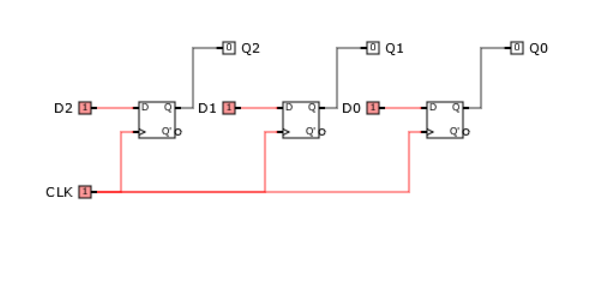
\includegraphics[scale=1]{Schema1.png}
\end{minipage}


\begin{figure}[H]
    \begin{minipage}{0.5\textwidth}
        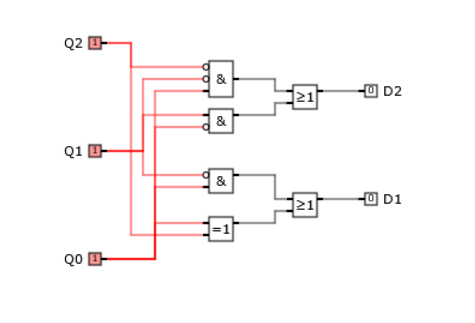
\includegraphics[scale=0.75]{Schema2.png}
    \end{minipage}
    \hfill
    \begin{minipage}{0.5\textwidth}
        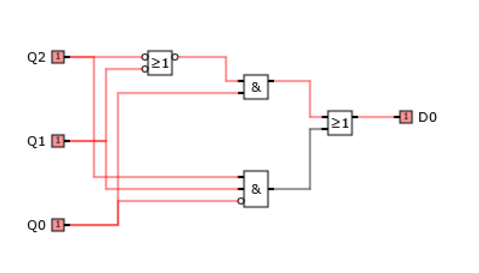
\includegraphics[scale=0.75]{Schema3.png}
    \end{minipage}
\end{figure}  

\newpage

\begin{figure}[h!]
    \begin{minipage}{0.75\textwidth}
        \begin{tikzpicture}
            \draw[thick] (0,0.35) arc[start angle=18, end angle=338, x radius=1cm, y radius=1cm];
            \draw[thick] (6,-0.35) arc[start angle=18, end angle=338, x radius=-1cm, y radius=-1cm];

            \node[circle, draw] (A) at (0,0) {0};
            \node[circle, draw] (B) at (6,0) {1};

            \draw[-] (0.25,0.25) -- (3,1);
            \draw[->] (3,1) -- (5.75,0.25);

            \draw[-] (0.25,-0.25) -- (3,-1);
            \draw[->] (3,-1) -- (5.75,-0.25);

            \node at (-1,0.25) {J=0};
            \node at (-1,-0.25) {K=0};
            \node at (-2.75,0.25) {J=0};
            \node at (-2.75,-0.25) {K=1};
            %
            \node at (7,0.25) {J=0};
            \node at (7,-0.25) {K=0};
            \node at (8.75,0.25) {J=0};
            \node at (8.75,-0.25) {K=1};
            %
            \node at (3,0.5) {J=1;K=0};
            \node at (3,-0.5) {J=0;K=1};
            %
            \node at (3,1.5) {J=1;K=1};
            \node at (3,-1.5) {J=1;K=1};
            
            \draw[->] (0.35,0.1) -- (5.65,0.1);
            \draw[->] (5.65,-0.1) -- (0.35,-0.1);
        \end{tikzpicture}  
    \end{minipage}
    \hfill
    \begin{minipage}{0.18\textwidth}
        \begin{tabular}{|c|c|c|c|}
            \hline
            Q & $Q^{'}$ & J & K \\ \hline
            0 & 0 & 0 & X \\ \hline
            0 & 1 & 1 & X \\ \hline
            1 & 0 & X & 1 \\ \hline
            1 & 1 & X & 0 \\ \hline
        \end{tabular}
    \end{minipage}
\end{figure}  

\begin{figure}[h!]
    \begin{minipage}{1\textwidth}
        \center{
            \begin{tabular}{|c|c|c|c|c|c|c|c|c|c|c|c|}
                \hline
                $Q_2$ & $Q_1$ & $Q_0$ & $Q_2^{'}$ & $Q_1^{'}$ & $Q_0^{'}$ & $J_2$ & $K_2$ & $J_1$ & $K_1$ & $J_0$ & $K_0$ \\ \hline
                0 & 0 & 0 & 0 & 1 & 0 & 0 & X & 1 & X & 0 & X  \\ \hline
                0 & 0 & 1 & 1 & 0 & 1 & 1 & X & 0 & X & X & 0  \\ \hline
                0 & 1 & 0 & 1 & 1 & 0 & 1 & X & X & 0 & 0 & X  \\ \hline
                0 & 1 & 1 & 0 & 0 & 1 & 0 & X & X & 1 & X & 0  \\ \hline
                1 & 0 & 0 & 0 & 1 & 0 & X & 1 & 1 & X & 0 & X  \\ \hline
                1 & 0 & 1 & 0 & 1 & 1 & X & 1 & 1 & X & X & 0  \\ \hline
                1 & 1 & 0 & 1 & 0 & 1 & X & 0 & X & 1 & 1 & X  \\ \hline
                1 & 1 & 1 & 0 & 1 & 0 & X & 1 & X & 0 & X & 1  \\ \hline
            \end{tabular}
        }
    \end{minipage}
\end{figure}  


\begin{figure}[h!]
    \begin{minipage}{0.5\textwidth}
        $K_2=Q_0+\bar{Q_1}$
        \begin{tikzpicture}
            \draw (0,0) grid (4,-2);
            \draw[-] (0,0) -- (-1,1);
            \node at (-0.75, 1.25) {$Q_2$};
            \node at (-0.75, 0.25) {$Q_1$};
            \node at (-0.25, 0.75) {$Q_0$};
            \draw (0,0) grid (4,-2);
    
            \draw[thick] (2, -1.5) ellipse (2cm and 0.5cm);
            \draw[thick] (4,0) arc[start angle=90, end angle=270, x radius=1cm, y radius=1cm];
            \draw[thick] (0,-2) arc[start angle=-90, end angle=90, x radius=1cm, y radius=1cm];

            \node at (0.5, -0.5) {X};
            \node at (1.5, -0.5) {X};
            \node at (2.5, -0.5) {0};
            \node at (3.5, -0.5) {1};
            %
            \node at (0.5, -1.5) {X};
            \node at (1.5, -1.5) {X};
            \node at (2.5, -1.5) {1};
            \node at (3.5, -1.5) {1};
            
            \node at (0.5, 0.5) {00};
            \node at (1.5, 0.5) {01};
            \node at (2.5, 0.5) {11};
            \node at (3.5, 0.5) {10};
        
            \node at (-0.5, -0.5) {00};
            \node at (-0.5, -1.5) {01};
        \end{tikzpicture}
    \end{minipage}
    \hfill
    \begin{minipage}{0.5\textwidth}
        $J_2=Q_1\bigoplus Q_0$
        \begin{tikzpicture}
            \draw (0,0) grid (4,-2);
            \draw[-] (0,0) -- (-1,1);
            \node at (-0.75, 1.25) {$Q_2$};
            \node at (-0.75, 0.25) {$Q_1$};
            \node at (-0.25, 0.75) {$Q_0$};
            \draw (0,0) grid (4,-2);
    
            \draw[thick] (2, -0.5) ellipse (1cm and 0.5cm);
            \draw[thick] (4,-1) arc[start angle=90, end angle=270, x radius=1cm, y radius=0.5cm];
            \draw[thick] (0,-2) arc[start angle=-90, end angle=90, x radius=1cm, y radius=0.5cm];

            \node at (0.5, -0.5) {0};
            \node at (1.5, -0.5) {1};
            \node at (2.5, -0.5) {X};
            \node at (3.5, -0.5) {X};
            %
            \node at (0.5, -1.5) {1};
            \node at (1.5, -1.5) {0};
            \node at (2.5, -1.5) {X};
            \node at (3.5, -1.5) {X};
            
            \node at (0.5, 0.5) {00};
            \node at (1.5, 0.5) {01};
            \node at (2.5, 0.5) {11};
            \node at (3.5, 0.5) {10};
        
            \node at (-0.5, -0.5) {00};
            \node at (-0.5, -1.5) {01};
        \end{tikzpicture}
    \end{minipage}
\end{figure}  

\begin{figure}[h!]
    \begin{minipage}{0.5\textwidth}
        $K_1=Q_2\bigoplus Q_0$
        \begin{tikzpicture}
            \draw (0,0) grid (4,-2);
            \draw[-] (0,0) -- (-1,1);
            \node at (-0.75, 1.25) {$Q_2$};
            \node at (-0.75, 0.25) {$Q_1$};
            \node at (-0.25, 0.75) {$Q_0$};
            \draw (0,0) grid (4,-2);
    
            \draw[thick] (1, -1.5) ellipse (1cm and 0.5cm);
            \draw[thick] (3, -0.5) ellipse (1cm and 0.5cm);

            \node at (0.5, -0.5) {X};
            \node at (1.5, -0.5) {0};
            \node at (2.5, -0.5) {1};
            \node at (3.5, -0.5) {X};
            %
            \node at (0.5, -1.5) {X};
            \node at (1.5, -1.5) {1};
            \node at (2.5, -1.5) {0};
            \node at (3.5, -1.5) {X};
            
            \node at (0.5, 0.5) {00};
            \node at (1.5, 0.5) {01};
            \node at (2.5, 0.5) {11};
            \node at (3.5, 0.5) {10};
        
            \node at (-0.5, -0.5) {00};
            \node at (-0.5, -1.5) {01};
        \end{tikzpicture}
    \end{minipage}
    \hfill
    \begin{minipage}{0.5\textwidth}
        $J_1=\bar{Q_0}+Q_2$
        \begin{tikzpicture}
            \draw (0,0) grid (4,-2);
            \draw[-] (0,0) -- (-1,1);
            \node at (-0.75, 1.25) {$Q_2$};
            \node at (-0.75, 0.25) {$Q_1$};
            \node at (-0.25, 0.75) {$Q_0$};
            \draw (0,0) grid (4,-2);
    
            \draw[thick] (2, -0.5) ellipse (2cm and 0.5cm);
            \draw[thick] (3, -1) ellipse (1cm and 1cm);

            \node at (0.5, -0.5) {0};
            \node at (1.5, -0.5) {1};
            \node at (2.5, -0.5) {X};
            \node at (3.5, -0.5) {X};
            %
            \node at (0.5, -1.5) {1};
            \node at (1.5, -1.5) {0};
            \node at (2.5, -1.5) {X};
            \node at (3.5, -1.5) {X};
            
            \node at (0.5, 0.5) {00};
            \node at (1.5, 0.5) {01};
            \node at (2.5, 0.5) {11};
            \node at (3.5, 0.5) {10};
        
            \node at (-0.5, -0.5) {00};
            \node at (-0.5, -1.5) {01};
        \end{tikzpicture}
    \end{minipage}
\end{figure}

\begin{figure}[h!]
    \begin{minipage}{0.5\textwidth}
        $K_0=Q_2Q_1$
        \begin{tikzpicture}
            \draw (0,0) grid (4,-2);
            \draw[-] (0,0) -- (-1,1);
            \node at (-0.75, 1.25) {$Q_2$};
            \node at (-0.75, 0.25) {$Q_1$};
            \node at (-0.25, 0.75) {$Q_0$};
            \draw (0,0) grid (4,-2);
    
            \draw[thick] (2.5, -1) ellipse (0.5cm and 1cm);

            \node at (0.5, -0.5) {X};
            \node at (1.5, -0.5) {X};
            \node at (2.5, -0.5) {X};
            \node at (3.5, -0.5) {X};
            %
            \node at (0.5, -1.5) {0};
            \node at (1.5, -1.5) {0};
            \node at (2.5, -1.5) {1};
            \node at (3.5, -1.5) {0};
            
            \node at (0.5, 0.5) {00};
            \node at (1.5, 0.5) {01};
            \node at (2.5, 0.5) {11};
            \node at (3.5, 0.5) {10};
        
            \node at (-0.5, -0.5) {00};
            \node at (-0.5, -1.5) {01};
        \end{tikzpicture}
    \end{minipage}
    \hfill
    \begin{minipage}{0.5\textwidth}
        $J_0=Q_2Q_1$
        \begin{tikzpicture}
            \draw (0,0) grid (4,-2);
            \draw[-] (0,0) -- (-1,1);
            \node at (-0.75, 1.25) {$Q_2$};
            \node at (-0.75, 0.25) {$Q_1$};
            \node at (-0.25, 0.75) {$Q_0$};
            \draw (0,0) grid (4,-2);
    
            \draw[thick] (2.5, -1) ellipse (0.5cm and 1cm);

            \node at (0.5, -0.5) {0};
            \node at (1.5, -0.5) {0};
            \node at (2.5, -0.5) {1};
            \node at (3.5, -0.5) {0};
            %
            \node at (0.5, -1.5) {X};
            \node at (1.5, -1.5) {X};
            \node at (2.5, -1.5) {X};
            \node at (3.5, -1.5) {X};
            
            \node at (0.5, 0.5) {00};
            \node at (1.5, 0.5) {01};
            \node at (2.5, 0.5) {11};
            \node at (3.5, 0.5) {10};
        
            \node at (-0.5, -0.5) {00};
            \node at (-0.5, -1.5) {01};
        \end{tikzpicture}
    \end{minipage}
\end{figure}

\begin{tikztimingtable}
    CLK       & LLHHLLHHLLHHLLHHLLHHLLHHLLHHLLHHLLHHLLHHLL \\
    $Q_2$     & LLLLLLHHHHHHHHLLLLLLLLHHHHSSHHHHLLLLSSHHLL \\
    $Q_1$     & LLHHHHHHHHLLLLHHHHLLLLLLLLSSLLLLHHHHSSHHHH \\
    $Q_0$     & LLLLLLLLLLHHHHHHHHHHHHHHHHSSLLLLLLLLSSHHLL \\
\end{tikztimingtable}\\
\begin{tikzpicture}[overlay, shift={(1, -1.5)}]
    \node[below] at (0, 5.25) {\#};
    \node[below] at (1.00, 5.25) {0};
    \node[below] at (2, 5.25) {2};
    \node[below] at (3.2, 5.25) {6};
    \node[below] at (4.4, 5.25) {5};
    \node[below] at (5.6, 5.25) {3};
    \node[below] at (6.8, 5.25) {1};
    \node[below] at (8, 5.25) {5};

    \node[below] at (9.75, 5.25) {4};
    \node[below] at (10.75, 5.25) {2};
    \node[below] at (12.35, 5.25) {7};
    \node[below] at (13, 5.25) {2};
    
    \node[rotate=90, anchor=north] at (-1, 2.5) {Semnale};
\end{tikzpicture}

\begin{figure}[h!]
    \begin{minipage}{1\textwidth}
        \center{
            \begin{tabular}{|c|c|c|c|c|c|c|c|c|}
                \hline
                $Q_2$ & $Q_1$ & $Q_0$ & $Q_2^{'}$ & $Q_1^{'}$ & $Q_0^{'}$ & $T_2$ & $T_1$ & $T_0$ \\ \hline
                0 & 0 & 0 & 0 & 1 & 0 & 0 & 1 & 0 \\ \hline
                0 & 0 & 1 & 1 & 0 & 1 & 1 & 0 & 0 \\ \hline
                0 & 1 & 0 & 1 & 1 & 0 & 1 & 0 & 0 \\ \hline
                0 & 1 & 1 & 0 & 0 & 1 & 0 & 1 & 0 \\ \hline
                1 & 0 & 0 & 0 & 1 & 0 & 1 & 1 & 0 \\ \hline
                1 & 0 & 1 & 0 & 1 & 1 & 1 & 1 & 0 \\ \hline
                1 & 1 & 0 & 1 & 0 & 1 & 0 & 1 & 1 \\ \hline
                1 & 1 & 1 & 0 & 1 & 0 & 1 & 0 & 1 \\ \hline
            \end{tabular}
        }
    \end{minipage}
\end{figure}  
\center{
    $T_2=\bar{Q_1}Q_0+Q_2\bar{Q_1}+\bar{Q_2}Q_1\bar{Q_0}+Q_2Q_0$
    \begin{tikzpicture}
        \draw (0,0) grid (4,-2);
        \draw[-] (0,0) -- (-1,1);
        \node at (-0.75, 1.25) {$Q_2$};
        \node at (-0.75, 0.25) {$Q_1$};
        \node at (-0.25, 0.75) {$Q_0$};

        \draw (0,0) grid (4,-2);

        \draw[thick] (3, -1.5) ellipse (1cm and 0.5cm);
        \draw[thick] (1.5, -0.5) ellipse (0.5cm and 0.5cm);
        \draw[thick] (3.5, -1) ellipse (0.5cm and 1cm);

        \draw[thick] (4,-1) arc[start angle=90, end angle=270, x radius=1cm, y radius=0.5cm];
        \draw[thick] (0,-2) arc[start angle=-90, end angle=90, x radius=1cm, y radius=0.5cm];

        \node at (0.5, -0.5) {0};
        \node at (1.5, -0.5) {1};
        \node at (2.5, -0.5) {0};
        \node at (3.5, -0.5) {1};
        %
        \node at (0.5, -1.5) {1};
        \node at (1.5, -1.5) {0};
        \node at (2.5, -1.5) {1};
        \node at (3.5, -1.5) {1};
        
        \node at (0.5, 0.5) {00};
        \node at (1.5, 0.5) {01};
        \node at (2.5, 0.5) {11};
        \node at (3.5, 0.5) {10};

        \node at (-0.5, -0.5) {00};
        \node at (-0.5, -1.5) {01};
    \end{tikzpicture}
}
\center{
    $T_1=Q_2\bar{Q_0}+\bar{Q_1}\bar{Q_0}+Q_2\bar{Q_1}+\bar{Q_2}Q_1Q_0$
    \begin{tikzpicture}
        \draw (0,0) grid (4,-2);
        \draw[-] (0,0) -- (-1,1);
        \node at (-0.75, 1.25) {$Q_2$};
        \node at (-0.75, 0.25) {$Q_1$};
        \node at (-0.25, 0.75) {$Q_0$};

        \draw (0,0) grid (4,-2);

        \draw[thick] (3, -0.5) ellipse (1cm and 0.5cm);
        \draw[thick] (1.5, -1.5) ellipse (0.5cm and 0.5cm);
        \draw[thick] (3.5, -1) ellipse (0.5cm and 1cm);

        \draw[thick] (4,0) arc[start angle=90, end angle=270, x radius=1cm, y radius=0.5cm];
        \draw[thick] (0,-1) arc[start angle=-90, end angle=90, x radius=1cm, y radius=0.5cm];

        \node at (0.5, -0.5) {1};
        \node at (1.5, -0.5) {0};
        \node at (2.5, -0.5) {1};
        \node at (3.5, -0.5) {1};
        %
        \node at (0.5, -1.5) {0};
        \node at (1.5, -1.5) {1};
        \node at (2.5, -1.5) {0};
        \node at (3.5, -1.5) {1};
        
        \node at (0.5, 0.5) {00};
        \node at (1.5, 0.5) {01};
        \node at (2.5, 0.5) {11};
        \node at (3.5, 0.5) {10};

        \node at (-0.5, -0.5) {00};
        \node at (-0.5, -1.5) {01};
    \end{tikzpicture}
}
\center{
    $T_1=Q_2\bar{Q_0}+\bar{Q_1}\bar{Q_0}+Q_2\bar{Q_1}+\bar{Q_2}Q_1Q_0$
    \begin{tikzpicture}
        \draw (0,0) grid (4,-2);
        \draw[-] (0,0) -- (-1,1);
        \node at (-0.75, 1.25) {$Q_2$};
        \node at (-0.75, 0.25) {$Q_1$};
        \node at (-0.25, 0.75) {$Q_0$};

        \draw (0,0) grid (4,-2);

        \draw[thick] (2.5, -1) ellipse (0.5cm and 1cm);

        \node at (0.5, -0.5) {0};
        \node at (1.5, -0.5) {0};
        \node at (2.5, -0.5) {1};
        \node at (3.5, -0.5) {0};
        %
        \node at (0.5, -1.5) {0};
        \node at (1.5, -1.5) {0};
        \node at (2.5, -1.5) {1};
        \node at (3.5, -1.5) {0};
        
        \node at (0.5, 0.5) {00};
        \node at (1.5, 0.5) {01};
        \node at (2.5, 0.5) {11};
        \node at (3.5, 0.5) {10};

        \node at (-0.5, -0.5) {00};
        \node at (-0.5, -1.5) {01};
    \end{tikzpicture}
}

\end{document}